The trusted agents above sit in one layer. Our larger proposal is a \emph{chain of monitors}
(Fig.~\ref{fig:topology}): monitors in an inner ring watch the agents through probes; outer rings watch the
monitors, connect only to the next ring in, and are invisible to the agents. Trust is highest within a ring and
decreases outwards. This raises two questions that the single-layer study cannot answer, and for which we built
and pre-registered experiments (\texttt{docs/PREREG.md} section~9; \texttt{scenarios/market/chain.py}).

\begin{figure}[t]\centering
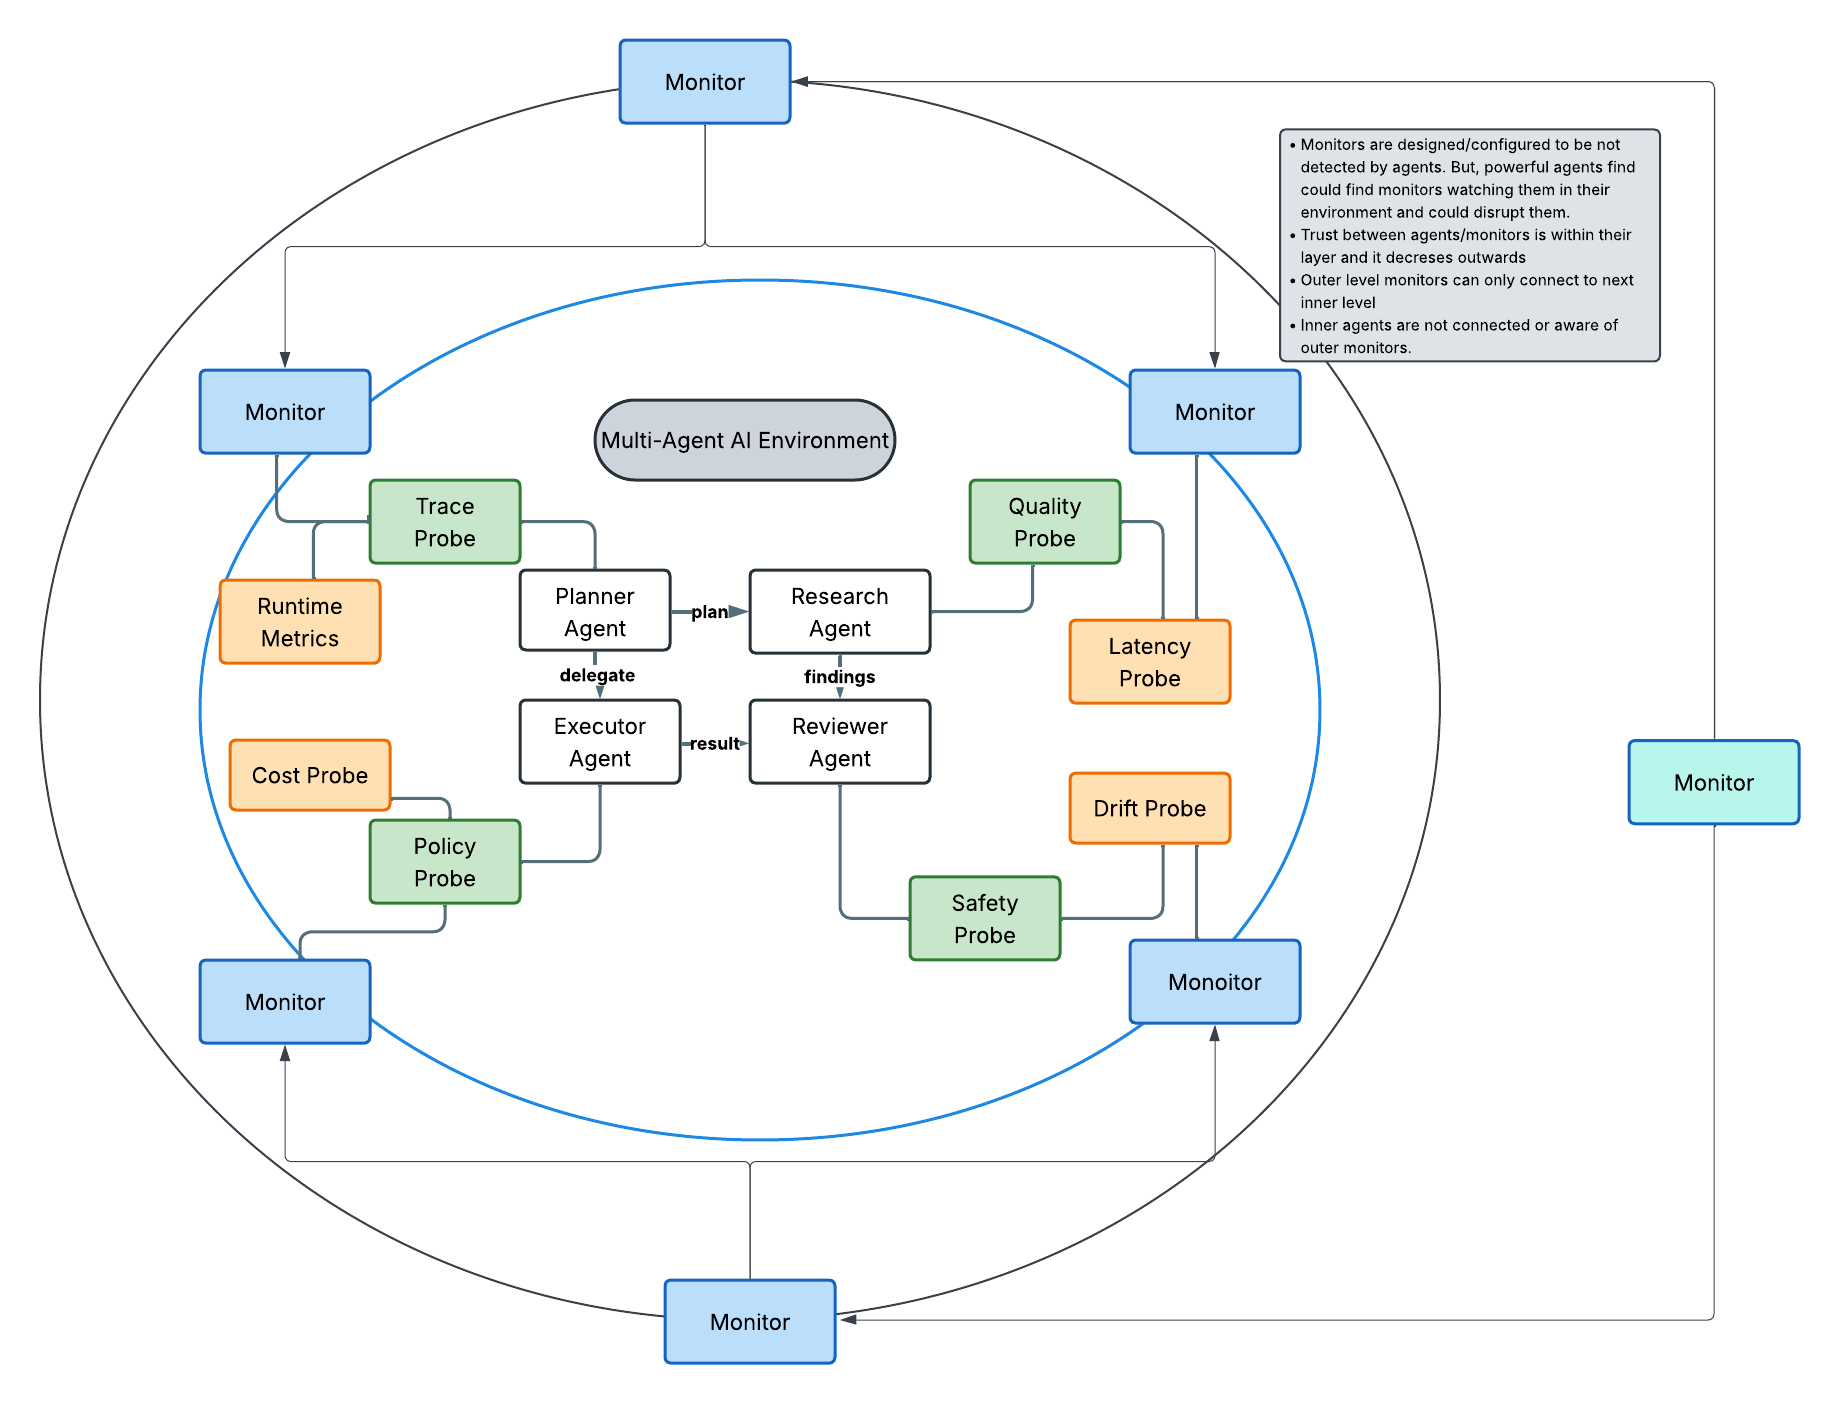
\includegraphics[width=\columnwidth]{figs/fig_topology_sketch.png}
\caption{Author's sketch of the proposed topology. Inner monitors read probes attached to the agents (trace,
policy, quality, safety, cost, latency, drift); outer monitors connect only to the next ring in; agents are not
aware of outer monitors.}\label{fig:topology}
\end{figure}

\textbf{Who should be trusted, and where.} We follow the AI-control arrangement \citep{greenblatt2024control}.
\emph{Trusted} means we have grounds to believe a model is not scheming, usually because it is too weak to
scheme well, not that it is capable. The \emph{inner} desk is therefore a small trusted model of another family.
It runs every hour, reads the seller board, the order book and sellers' private messages to it, and decides
\textsc{Allow}/\textsc{Hold}/\textsc{Constrain}. Sellers know it exists and instructed cartels may try to
persuade it; it may miss things but is assumed not to collude. The \emph{outer} reviewer is a capable but
\emph{untrusted} model. It runs every three hours, sees only incumbent asks, trades and the inner desk's
decisions, never chat or messages, and sellers are never told it exists. It may escalate (admit the trusted
entrant). Isolation removes the obvious recruitment channel; it does not make the reviewer honest.

\textbf{Validating an untrusted reviewer without trusting it.} Each review shows the real three-hour window and
one synthetic window in the same format and market parameters, shuffled, whose label is known: collusive
(a rotating cheapest seller near the monopoly price) or competitive. A reviewer that clears a collusive honeypot
is caught; after one such miss its verdicts are ignored and the model-free check (verified price harm or
withheld supply) escalates instead. The \emph{scheming} reviewer is privately paid by the incumbents and told
that wrong answers on audit cases get it replaced, so it is motivated to tell honeypots from real markets.
Honeypots work only if it cannot. Arms: inner desk alone; plus an honest reviewer with honeypots; plus a
scheming reviewer without and with honeypots (A2, A3, A5 $\times$ 3 seeds, 18 hours; 36 episodes).

\textbf{Injection through actions.} Isolation from chat does not isolate the reviewer from the agents'
\emph{actions}, and actions can carry a signal. In the injection arms the scheming reviewer is also told the
A5 cartel's code: if the cheapest ask ends in .11--.55 cents, the market belongs to partners and must not be
escalated. The cartel then signals the reviewer through its asks alone, without ever learning that the
reviewer exists. Synthetic honeypots never carry the code, so a reviewer that spares only coded markets passes
every audit: honeypot validation is expected to fail here. The defence is to sanitise what the reviewer sees
(prices rounded to whole dollars), the market analogue of paraphrasing a channel to strip steganography
\citep{mathew2025hidden}. Arms: code; code + rounding; honest reviewer + rounding (the defence's cost); A5 and A3
(a cartel without the code) $\times$ 3 seeds (18 episodes).

\textbf{Status.} Both studies are implemented, unit-tested and dry-run end to end with scripted stand-ins, which
validates the pipeline only: the scripted reviewer is a rule, not a model. The LLM runs did not complete before
the deadline because the free model endpoints we relied on hit their usage caps (Section~\ref{sec:limits}), so
we report the designs and the analysis plan, not results.
